\documentclass[10pt]{beamer}

\usepackage[american]{babel}
\usepackage[utf8]{inputenc}
%\usepackage{soul}
\usepackage{amsmath}
\usepackage{amssymb}
\usepackage{textcomp}
\usepackage{listings}
\lstset{
  language=haskell,
  upquote=true,
  basicstyle=\ttfamily,          % print whole listing in typewriter
  keywordstyle=\color{blue}\bfseries, % bold blue keywords
  %identifierstyle=,           % nothing happens
  commentstyle=\color{green}, % green comments
  stringstyle=\color{red},      % typewriter type for strings
  showstringspaces=false     % no special string spaces
}
%\usepackage[all]{xy}
\usepackage{tikz}
%\usetikzlibrary{arrows,shapes,automata}
\usepackage{graphicx}
%\usepackage[bibstyle=beamer,citestyle=authoryear-comp,doi=false,isbn=false,eprint=false,maxnames=10]{biblatex}
%\bibliography{../defeo}
\usepackage{../mysymbols}
\usepackage{array}

% \usepackage[T1]{fontenc}
% \renewcommand{\rmdefault}{pplx}
% \renewcommand{\sfdefault}{uop}
% \usepackage[T1]{eulervm}


\mode<presentation>{%
  \usetheme[]{Madrid}
  \usefonttheme{professionalfonts}
  \usecolortheme{crane}
% \usecolortheme{rose}
}


\title{Fast Algorithms for Towers of Finite Fields and Isogenies}
\author{Luca~De~Feo}
\institute[LIX \& INRIA Saclay]{LIX, École Polytechnique \& INRIA Saclay, Projet TANC}
\date[December 13, 2010]{December 13, 2010\\École Polytechnique, Palaiseau}


\AtBeginSection[]
{
  \begin{frame}<beamer>
    \frametitle{Plan}
    \tableofcontents[currentsection]
  \end{frame}
}

\begin{document}

\begin{frame}
  \titlepage
%   
\includegraphics[height=2em]{../logos/x-color.pdf}
%   \hfill
%   
\includegraphics[height=2em]{../logos/lix-color.pdf}
%   \hfill
%   
\includegraphics[height=2em]{../logos/inria-color.pdf}
\end{frame}

%%
%%

\begin{frame}[fragile]
  \frametitle{The Discrete Logarithm Problem}
  
  \begin{columns}
    \begin{column}{0.4\textwidth}
      \begin{tikzpicture}
        \begin{scope}
          \foreach \alpha in {0,...,4} {
            \filldraw (-65-25*\alpha:2) circle (2pt);
          }
          \foreach \alpha in {0,...,3} {
            \draw[->] (-65-25*\alpha:2) arc (-65-25*\alpha:-85-25*\alpha:2);
            \draw (-90-25*\alpha:2.3) node {$g^\alpha$};
          }
          \draw (-65:2.3) node {$g^{n-1}$};
          \draw[densely dotted,gray] (-65:2) arc (-65:195:2);
          \draw (0,0) node {\Large $G=\langle g\rangle$};
        \end{scope}
        
        \begin{uncoverenv}<2->
          \begin{scope}[yshift=-3cm]
            \foreach \alpha in {0,...,4} {
              \filldraw (-65-25*\alpha:2) circle (2pt);
            }
            \foreach \alpha in {0,...,3} {
              \draw[->] (-65-25*\alpha:2) arc (-65-25*\alpha:-85-25*\alpha:2);
              \draw (-90-25*\alpha:2.3) node {$\alpha$};
            }
            \draw (-65:2.3) node {$n-1$};
            \draw[densely dotted,gray] (-65:2) arc (-65:48:2);
            \draw[densely dotted,gray] (132:2) arc (132:195:2);
            \draw (0,-0.5) node {\Large $\Z/n\Z$};
          \end{scope}
        \end{uncoverenv}
        
        \begin{uncoverenv}<3->
          \foreach \alpha in {0,...,4}
          \draw[dashed,red] (-65-25*\alpha:2) -- ++(0,-3cm);
        \end{uncoverenv}
      \end{tikzpicture}
    \end{column}
    \begin{column}{0.6\textwidth}
      \begin{block}{Exponentiation in a cyclic group}
        Let $G=\langle g\rangle$ be a cyclic group of order $n$.
        Define
        \begin{align*}
          \exp_g : \Z/n\Z &\ra G\text{,}\\
          x&\mapsto g^x\text{.}
        \end{align*}
      \end{block}

      \begin{block}<2->{Discrete logarithm} $\exp_g$ is an
        isomorphism. Its inverse is called \emph{discrete logarithm}.
        \begin{align*}
          \log_g : G &\ra \Z/n\Z\text{,}\\
          g^x&\mapsto x\text{.}
        \end{align*}

        \begin{uncoverenv}<3-> Computing it is called the
          \alert{\emph{Discrete Logarithm Problem}} (DLP) of $G$.
        \end{uncoverenv}
      \end{block}
    \end{column}
  \end{columns}
\end{frame}

%%
{\setbeamertemplate{navigation symbols}{}
\begin{frame}
  \frametitle{Elliptic curve cryptography}

  \begin{block}{Finite field based cryptography}
    \begin{itemize}
    \item The discrete log in $\F_p^\ast$ is widely used in
      cryptography (El Gamal, DSA, \dots).
    \item However, NIST\footfullcite{nist07} recommends $\log_2p=1024$
      for an 80-bit security level.
    \end{itemize}
  \end{block}

  \begin{columns}
    \begin{column}{0.4\textwidth}
      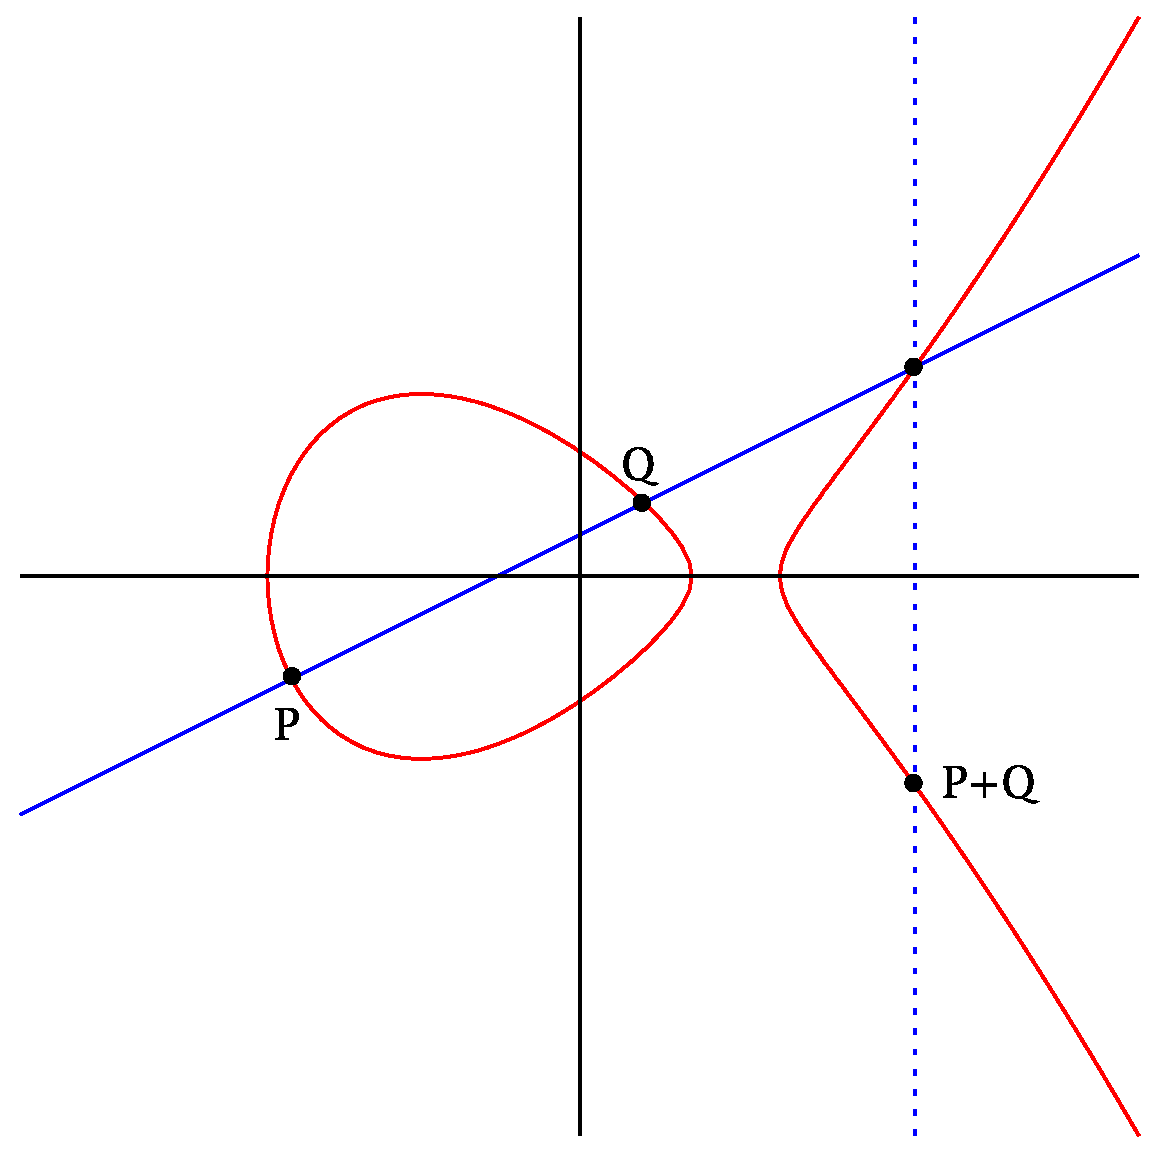
\includegraphics[width=\textwidth]{../isogeny/ec-add.pdf}
    \end{column}
    \begin{column}{0.6\textwidth}
      \begin{block}{Elliptic curve cryptography}
        The set of points of an elliptic curve is endowed with a group
        law via the chord-and-tangent law.
        
        \smallskip

        \begin{description}
        \item[Weierstrass form:] $E : y^2 = x^3 + ax + b$;
        \item[Hasse bound:] $\card{E(\F_q)} \sim q$.
        \end{description}

        \smallskip

        Comparatively, NIST recommends $\log_2q=160$ for the same
        security level.
      \end{block}
    \end{column}
  \end{columns}
\end{frame}
}


\end{document}


% Local Variables:
% mode:flyspell
% ispell-local-dictionary:"american"
% mode:TeX-PDF
% mode:reftex
% End:
%
% LocalWords:  Isogeny abelian isogenies hyperelliptic supersingular Frobenius
% LocalWords:  isogenous
